\documentclass[11pt]{article}

\usepackage{latexsym}
\usepackage[linesnumbered, vlined, ruled]{algorithm2e}
\oddsidemargin=0.0in
\evensidemargin=0.0in
\headheight=0.0in
\topmargin=-0.40in %0.35
\textheight=9.0in %9.1in
\textwidth=6.5in   %6.55in
\usepackage{fullpage}
\usepackage{listings}
\usepackage{graphicx}
\usepackage{xfrac}
\usepackage{mathtools}
\DeclarePairedDelimiter{\ceil}{\lceil}{\rceil}
\DeclarePairedDelimiter\floor{\lfloor}{\rfloor}

\newcommand{\mybox}[1]{\fbox{\begin{minipage}{\linewidth} #1 \end{minipage}}}

% \graphicspath{ {./images/} }

\begin{document}
\baselineskip=14.0pt

\title{CS5050 \textsc{Advanced Algorithms}
\\{\Large Spring Semester, 2018}
\\ Assignment 3: Prune and Search
\\ {\bf Philip Nelson}
\\ {\large Worked with: Ammon Hepworth, Raul Ramirez, Hailey Maxwell, and Jack Kiefer}}
\date{}

\maketitle

\vspace{-0.7in}

\begin{enumerate}
\item % Problem 1
{\bf (20 points)}
Peak of a unimodal array.

  \begin{description}
  \item[1. Algorithm Description]

    The algorithm \textit{peak} finds the peak of a unimodal array, $A$, in $O(\log{n})$ making use of a prune and search algorithm similar to binary search. The algorithm begins by calculating the midpoint of the array, It checks if the element to the right is less than it and the element to the left is greater. If this is the case, then the midpoint is the peak. If, however, this is not the case, then it will determine whether the slope is positive or negative. Imagine if the value of the elements of $A$ were plotted against their indices. If the current element is not the peak, then the peak must be ``uphill'' from it and it can ignore the points ``downhill''. The next point to be checked is halfway between the current midpoint and the ``uphill'' side, until the peak is found.

  \item[2. Pseudocode]
    \textit{peak}
  \begin{lstlisting}[language=C++,
                     % directivestyle={\color{black}}
                     % emph={int,char,double,float,unsigned},
                     % emphstyle={\color{blue}}
                    ]
  template <typename T>
  int peak(std::vector< T > A, int start, int end)
  {
    // no peak exists
    if (start > end)
      return -1;

    auto mid = (start + end) / 2;

    // peak located
    if (A[mid - 1] < A[mid] && A[mid] > A[mid + 1])
      return mid;

    // positive slope
    if (A[mid - 1] < A[mid] && A[mid] < A[mid + 1])
      return peak(A, mid + 1, end);

    // negative slope
    if (A[mid - 1] > A[mid] && A[mid] > A[mid + 1])
      return peak(A, start, mid - 1);
  }
  \end{lstlisting}
  \item[3. Time Analysis]
    The algorithm \textit{peak} finds the peak of a unimodal array, $A$, in $O(\log{n})$. It is capable of doing this because each time a point is examined, half of the remaining elements are pruned. This means that the recurrence is $T(n) = T(\frac{n}{2}) \Rightarrow T(n) = \log(n)$.

  \end{description}

\item % Problem 2
{\bf (20 points)}
In the SELECTION algorithm we studied in class, the input numbers are divided into groups of five. Will the algorithm still work in linear time if they are divided into groups of seven? Please justify your answer.

\mybox{
The selection algorithm partitions a set $A$ into two sets $A_1$ and $A_2$. In order to pick a pivot, selection uses a method of choosing a median of medians. If groups of seven are used, instead of five, the median of medians will still guarantee that a constant portion of the elements of $A$ will go in sets $A_1$ and $A_2$. As shown below in Figure \ref{fig:7groups}, we can see that both $A_1$ and $A_2$ will have at least $\frac{n}{7}\cdot\frac{1}{2}\cdot4 = \frac{4}{14}n$ elements and at most $n-\frac{4}{14}n=\frac{10}{14}n$. Therefore, in the worst case, one partition of $A$ will have at least $\frac{4}{14}n$ elements. Since $\frac{4}{14}n$ is a constant percentage of $n$, not just a constant number, the selection algorithm will still have a time complexity of $O(n)$.

This idea can be further expanded to any number of elements $e$. The smallest that a partition of $A$ could be is $\frac{n}{e}\cdot\frac{1}{2}\cdot\ceil{\frac{e}{2}} = \frac{1}{2e}\ceil{\frac{e}{2}}n$ elements. In like fashion, this is a constant percentage of $n$, therefore the algorithm can run in linear time.
}

\begin{figure}[!htbp]
     \centering
     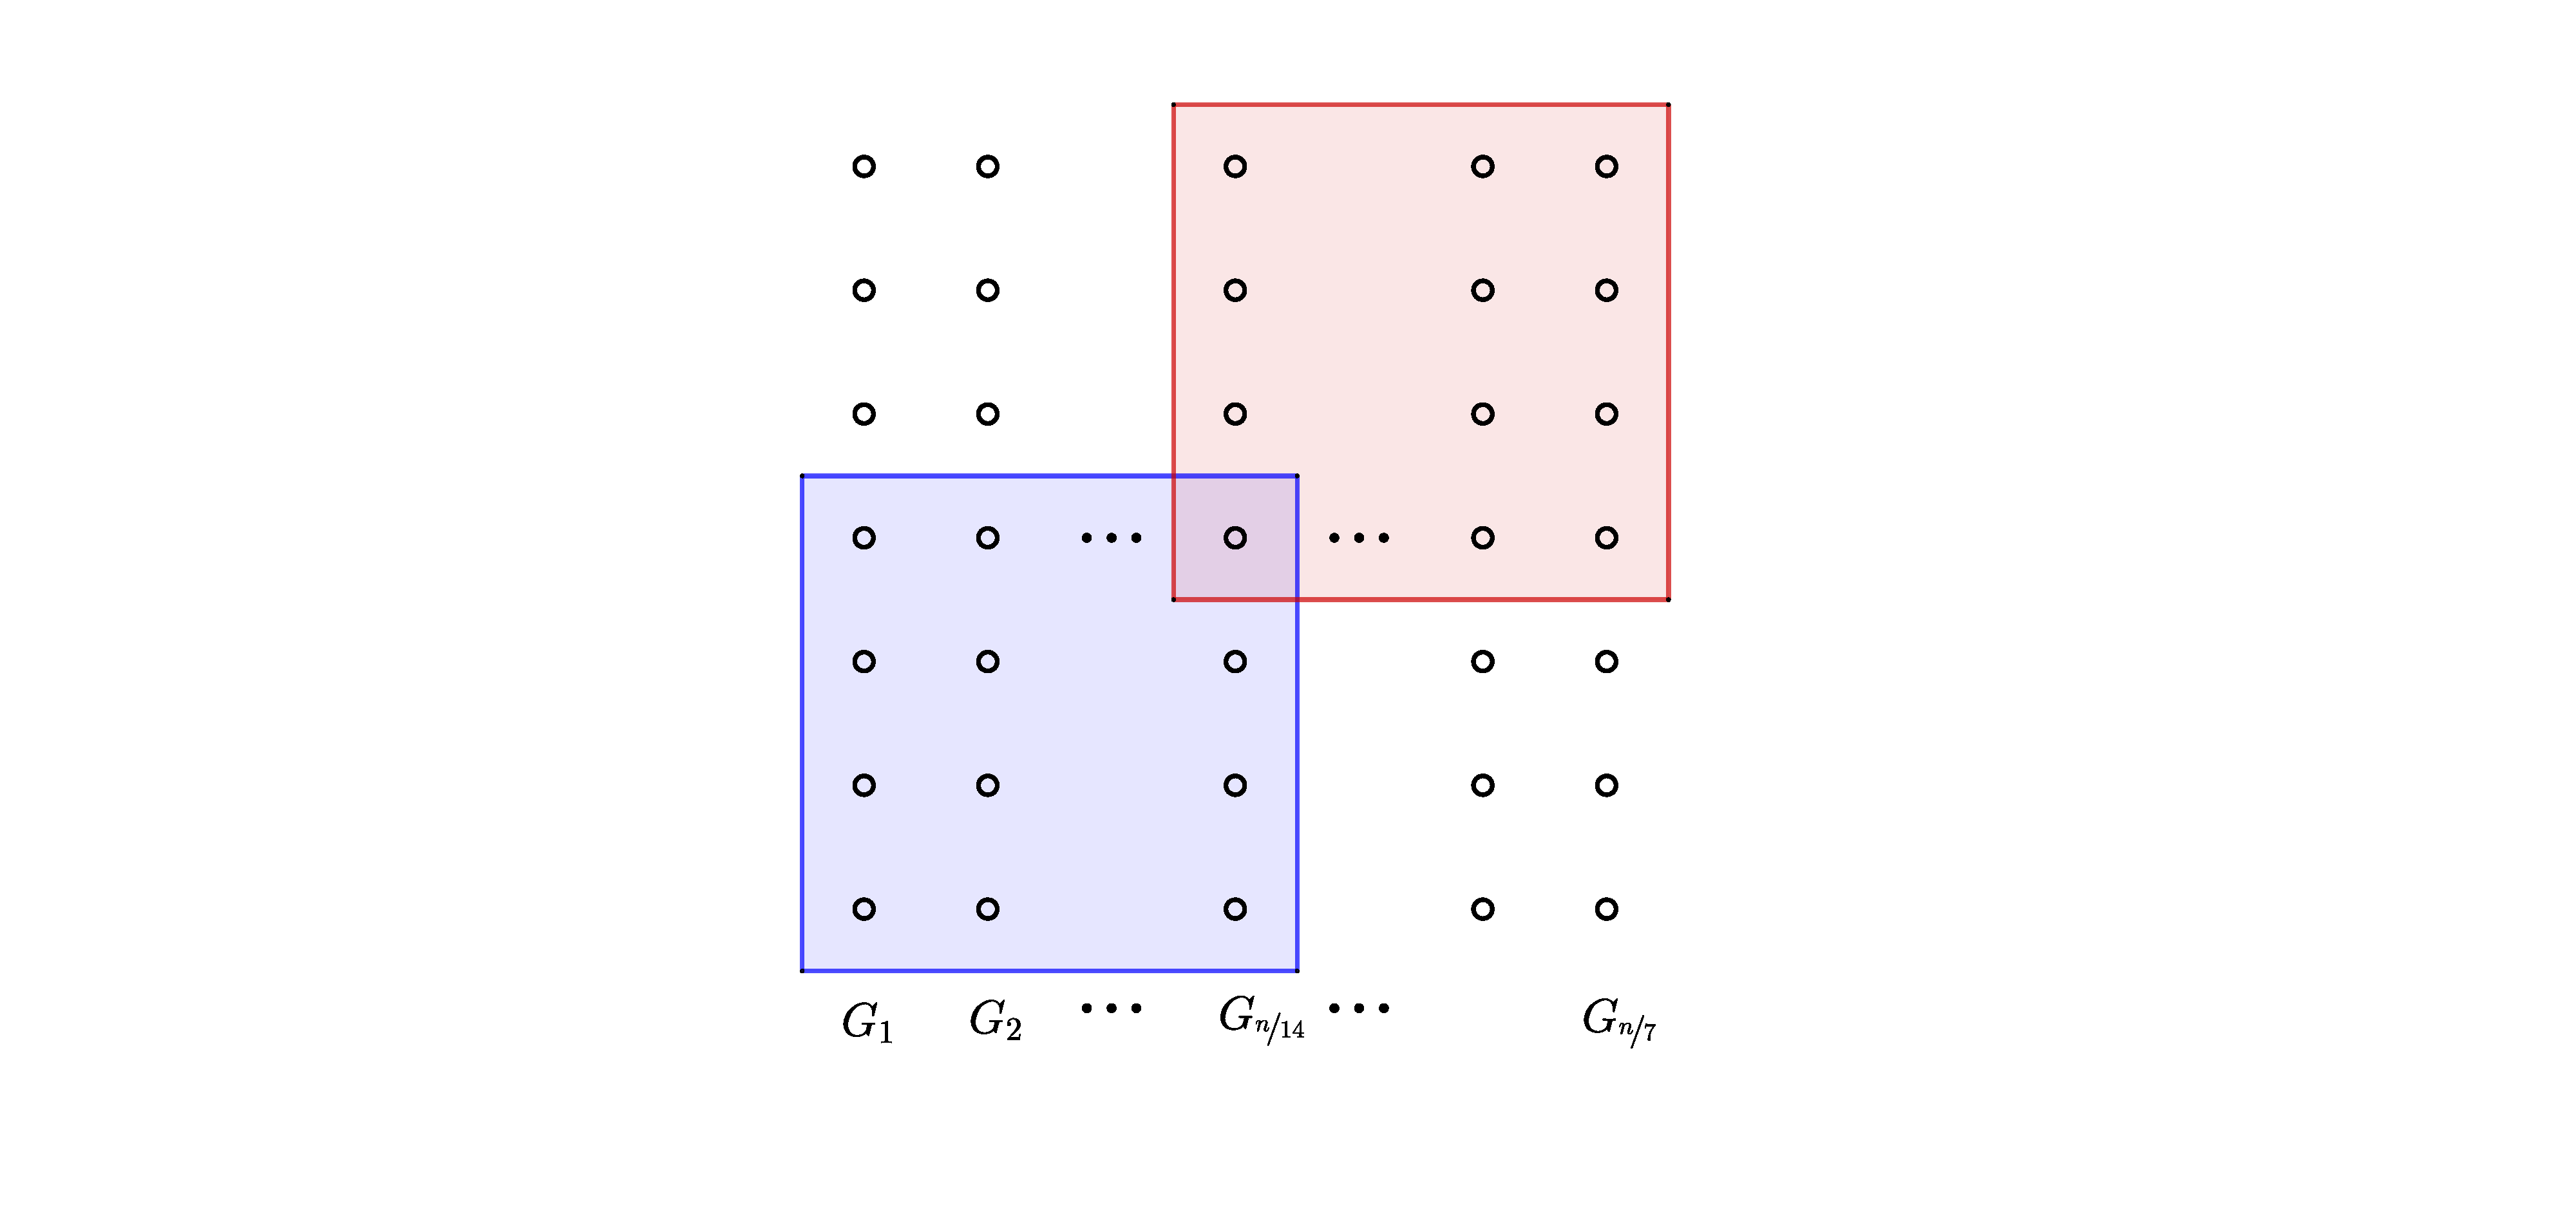
\includegraphics[width=\linewidth]{problem2.pdf}
     \caption{Groups of 7}\label{fig:7groups}
\end{figure}

  \newpage
\item % Problem 3
{\bf (20 points)}
Design an $O(n)$ time algorithm to compute an optimal location for the main pipeline.

  \begin{description}
  \item[1. Algorithm Description]

    The algorithm \textit{layPipe} finds the optimal location to place the main pipeline given an array, $A$, of well locations. It will accomplish this by selecting the median $y$ value from all the wells.

  \item[2. Pseudocode]
    \textit{layPipe}
  \begin{lstlisting}[language=C++,
                     % directivestyle={\color{black}}
                     % emph={int,char,double,float,unsigned},
                     % emphstyle={\color{blue}}
                    ]
  template < typename T >
  int layPipe(std::vector< T > A)
  {
    // collect all the y coordinates
    std::vector< T > ys;
    for(auto && p : A)
      ys.push_back(p.y);

    // use selection to find the median y value
    auto y = selection(ys, ys.size()/2);

    // place pipeline at the median y value
    return y;
  }
  \end{lstlisting}
  \item[3. Time Analysis]
    The algorithm \textit{layPipe} finds the optimal location to place the main pipeline given an array, $A$, of well locations. The algorithm begins by doing one linear scan to separate the $y$ values into an array which takes $O(n)$ time. Then it uses the \textit{selection} algorithm to choose the median $y$ value, which also takes $O(n)$ time. Since \textit{layPipe} does $2n$ work to find the location of the main pipeline, it's time complexity is $O(n)$.
  \item[4. Correctness]
    The main pipeline can be laid exactly on the $y$ value of the median well because the optimal location for the pipe will place the same number of wells on either side of the main pipeline.

    For the case that there are an odd number of wells, the main pipeline will run directly over the well with the median $y$ value. If you were to shift the main pipeline up one unit, for example, you would be moving the pipeline closer to $\floor{\frac{n}{2}}$ wells but further from $\ceil{\frac{n}{2}}$ wells. Since $n$ is odd, this means the pipeline is moving away from one more well than it is moving closer to, therefore, for every unit it moves, it adds one more unit of total spur pipeline.

    For the case that there are an even number of wells, there will not be one single median well but two. Lets call the $y$ values for these two median wells $y_1$ and $y_2$. As long as the pipeline is placed at a $y_p$ such that $y_1 \leq y_p \leq y_2$ the total spur pipeline is minimized. If the main pipeline is moved around within the range $[y_1, y_2]$ there are an equal number of wells on either side so the change in total spur pipeline is not affected.
  \end{description}

  \newpage
\item % Problem 4
{\bf (30 points)}
Here is a generalized version of the selection problem, called {\em multiple selection}. Let $A[1\cdots n]$ be an array of $n$ numbers. Given a sequence of $m$ sorted integers $k_1, k_2,\ldots, k_m$, with $1\leq k_1<k_2<\cdots<k_m\leq n$, the {\em multiple selection problem} is to find the $k_i$-th smallest number in $A$ for all $i=1,2,\ldots,m$. For simplicity, we assume that no two numbers of $A$ are equal.

For example, let $A=\{1, 5, 9, 3, 7, 12, 15, 8, 21\}$, and $m=3$ with
$k_1 = 2$, $k_2 = 5$, and $k_3=7$. Hence, the goal is to find the 2nd,
the $5$-th, and the $7$-th smallest numbers of $A$, which are $3$,
$8$, and $12$, respectively.

\begin{enumerate}
  \item % a) n log n
  Design an $O(n\log n)$ time algorithm for the problem. {\hfill \bf (5 points)}

  \mybox{
    The trivial solution is to sort the array and do a single linear scan to find the $k$-smallest elements. Sorting can be done in $O(n \log n)$ and the linear scan will take an additional $n$ work. Since $n \log n$ is the dominating term, the algorithm's time complexity is $O(n \log n)$.
}

  \item % b) nm
  Design an $O(nm)$ time algorithm for the problem. {\hfill \bf (5 points)}

  \mybox{
    The \textit{selection} algorithm can find the $k^{th}$ smallest element in $O(n)$ time. If there are $m$ elements to locate, we can simple employ the \textit{selection} algorithm for each one. The algorithm will do $n$ work $m$ times which is time complexity $O(nm)$.
}

  \item % c) n log m
  Improve your algorithm to $O(n\log m)$ time. {\hfill \bf (20 points)}

  \mybox{
    In order to achieve multiple selection in $O(n \log m)$ the algorithm will begin by finding the $k_{mid}$ element. Because all the $k$'s are sorted, once we have found the $k_{mid}$ we will have the following situation,

    \[A_1 < k_{mid} < A_2\]

    where the $\{k_1, \ldots, k_{mid-1}\} \in A_1$ and $\{k_{mid+1}, \ldots, k_{m}\} \in A_2$. The algorithm then calls the function again with $A_1$ and $\{k_1, \ldots, k_{mid-1}\}$, and $A_2$ and $\{k_{mid+1}, \ldots, k_{m}\}$. It will need to divide the array of $k$'s $\log m$ times and at each level, there will be $n$ work done. For this reason, the time complexity will be $O(n \log m)$.
}

\end{enumerate}


\end{enumerate}

{\bf Total Points:} 90

\end{document}
